\documentclass[./\jobname.tex]{subfiles}
\begin{document}
\section {Experiment 2: Adaptive Number of Kernels}
\label{chap:experimet_2}
Although the parallel algorithm is effectively faster, the quality of the achieved solution is still not good enough. A common inaccuracy, especially with the testbed \gls{pde} 0A is that not all Gauss ``bumps'' are represented in the approximation.

\subsection{Hypotheses}
The idea tested here is an adaptive scheme for the number of kernels used. This new concept requires a convergence based halting criterion in the JADE algorithm. The algorithm is extended by a so called ``state detector''. Ideally, the state detector should stop the overall optimisation loop as soon as the algorithm has converged and before the function evaluation budget is exceeded. Generally, this is done by checking if the function value has not changed for a certain amount of generations. The state detector introduces a new parameter. The \gls{dt} represents the number of generations over which the best function value must remain unchanged. It can also be thought of as a buffer-time that allows the \gls{de} parameters F and CR to self-adapt. Further, the minError parameter has a new purpose. This is the minimal difference that the function value is allowed to change over \gls{dt} generations. The new paJADE is wrapped into the memetic framework. A flowchart of the process in shown in figure \ref{fig:uml_flow_adaptive_scheme}. The algorithm always starts with one kernel. From there on, the number of kernels is increased. After the ``state detector'' has stopped the paJADE, the \gls{ds} is employed on the best individual. If the last JADE/DS cycle was able to improve the function value, it is assumed that the best solution for that dimensionality is found. Thus, to further improve the approximation quality, the number of kernels must be increased. If the function value could not be decreased, a restart around the previous best population is performed. 
\begin{figure}[H]
	\centering
	\noindent\adjustbox{max width=0.9\linewidth}{
		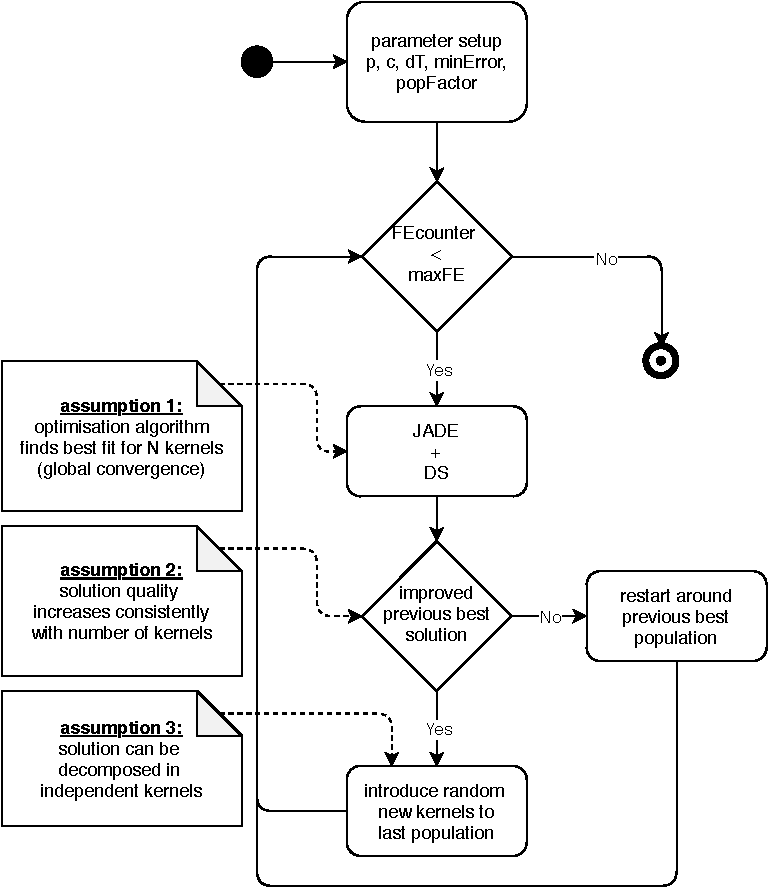
\includegraphics[width=\textwidth]{../../code/uml_diag/adaptive_kernels_flowchart.pdf}
	}
	\unterschrift{Flowchart of the adaptive kernel scheme.}{}{}
	\label{fig:uml_flow_adaptive_scheme}
\end{figure}
This adaptive scheme operates under 3 strong assumptions. To reduce their possible negative impact, corresponding counter-strategies are implemented. 
\begin{itemize}
	\item \underline{\textbf{Assumption 1:}} The optimisation algorithm (JADE + \gls{ds}) finds (a close approximation to) the global optimum. This would be the best approximation of the solution by $N$ kernels. Obviously, this property is not necessarily true. To counteract this assumption, restarts are performed. 
	\item \underline{\textbf{Assumption 2:}} The theoretically best achievable solution quality increases with the number of kernels. After a maximum number of kernels is reached, the quality can not be surpassed. Based on this assumption, the algorithm starts with one kernel and the dimensionality increases by only one kernel at a time. Generally, the maximum number of kernels is not known except for \gls{pde} 0A and \gls{pde} 6. 
	\item \underline{\textbf{Assumption 3:}} The best approximation of e.g. 3 kernels to a particular problem is independent of the best approximation by 4 kernels. This means that from 3 to 4 kernels simply a new kernel is introduced while not altering the other 3. Again, this is not true for every \gls{pde}. Preliminary experiments on \gls{pde} 0A have confirmed this assumption, while on \gls{pde} 2 the solution can not simply be decomposed into independent kernels. 
	In this algorithm, the first kernels are allowed to change. When introducing a new random kernel, it is simply appended to the ever evolving $\mathbf{p_{apx}}$ vector. Thus, the search for the 4th kernel starts where the best approximation for 3 kernels was found, but since the earlier kernels are allowed to readapt, other solutions can be retrieved.
\end{itemize} 
\subsection{Experiment Setup}
Again, as in the experiments before, machine 1 runs at $10^4$ \gls{nfe} and machine 2 performs $10^6$ \gls{nfe}. The number of kernels is adapted, but the algorithm starts with 1 \gls{gak}. Thus, the dimension is 4 and the population size is 8. The population size gets corrected if the number of kernels changes. The two new parameters \gls{dt} and minError must be set. The minError is again set to 0. The delay time \gls{dt} is set to 100. This choice is rather arbitrary and depending on the \gls{pde}, different values might be more successful. However, this property is not analysed in the current experiment.

\subsection{Results}
\label{chap:results_ex2}
The table \ref{tab:compare_mpj_mpja_10^6} shows the L2 norm data obtained by the adaptive JADE and compares them against the results from the parallel JADE. The Wilcoxon test indicates mixed results. The adaptive kernel scheme works fine on the \gls{pde} 0A, but it also produces significantly worse results on the problems \gls{pde} 2, 3, 4 and 7. 

\begin{table}[h]
	\centering
	\noindent\adjustbox{max width=\linewidth}{
		\begin{tabular}{|c|c|c|c|c|l|}
			
			\hline
			\rowcolor[HTML]{\farbeTabA}
			
			Algorithm & \multicolumn{2}{|c|}{parallel JADE $10^6$ \gls{nfe}} & \multicolumn{2}{|c|}{adaptive JADE $10^6$ \gls{nfe}} & \\ \hline
			stat & mean & median & mean & median & Wilcoxon Test \\ \hline \hline
			\gls{pde} 0A & 0.6939 $\pm$ 0.6635 & 0.9243 & 9.694E-16 $\pm$ 1.486E-16 & 9.255E-16 & sig. better \\ \hline
			\gls{pde} 0B & 0.2809 $\pm$ 0.3071 & 0.2035 & 0.2380 $\pm$ 0.0572 & 0.2607 & unsig. undecided \\ \hline
			\gls{pde} 1 & 0.0239 $\pm$ 0.0467 & 0.0146 & 0.0116 $\pm$ 0.0061 & 0.0084 & unsig. better \\ \hline
			\gls{pde} 2 & 0.0300 $\pm$ 0.0157 & 0.0255 & 0.0735 $\pm$ 0.0358 & 0.1034 & sig. worse \\ \hline
			\gls{pde} 3 & 0.0371 $\pm$ 0.0206 & 0.0295 & 0.1731 $\pm$ 0.0395 & 0.1822 & sig. worse \\ \hline
			\gls{pde} 4 & 0.0505 $\pm$ 0.0121 & 0.0481 & 0.0707 $\pm$ 0.0053 & 0.0720 & sig. worse\\ \hline
			\gls{pde} 5 & 1.2030 $\pm$ 0.0465 & 1.2053 & 122.6312 $\pm$ 372.5676 & 1.1643 & unsig. undecided \\ \hline
			\gls{pde} 6 & 0.5814 $\pm$ 1.3550 & 1.266E-17 & 0.4428 $\pm$ 1.0980 & 1.266E-17 & unsig. undecided \\ \hline
			\gls{pde} 7 & 0.0228 $\pm$ 0.0025 & 0.0226 & 0.0513 $\pm$ 0.0442 & 0.0231 & sig. worse \\ \hline
			\gls{pde} 8 & 0.2167 $\pm$ 0.0017 & 0.2169 & 0.2144 $\pm$ 0.0044 & 0.2128 & unsig. better \\ \hline
			\gls{pde} 9 & 0.0426 $\pm$ 0.0115 & 0.0463 & 0.0483 $\pm$ 0.0149 & 0.0468 & unsig. worse \\ \hline
			
		\end{tabular}
	}
	\unterschrift{Comparison of the achieved L2 norm by the pJADE and the paJADE at $10^6$ \gls{nfe}.}{}{}
	\label{tab:compare_mpj_mpja_10^6}
\end{table}

\subsection{Discussion}
\subsubsection{PDE 0A}
\label{chap:ex2_discussion_pde0a}
As noted before, the testbed \gls{pde} is especially designed to be solved by 5 \gls{gak}. The common problem, that not all kernels are established, is solved by the adaptive strategy. All 20 replications generate at least 5 kernels. However, some solutions are composed of 6 kernels, but this has only a limited effect on the numerical value of the solution quality. Generally, 6 kernels tend to produce worse solutions. The results by the \gls{ci} solver can even compete with the \gls{fem} solver results from table \ref{tab:fem_sol_quality}.

\subsubsection{Significantly Worse Quality}
\label{chap:pde 2 3 4 7} 
The Wilcoxon significance test of table \ref{tab:compare_mpj_mpja_10^6} shows that the adaptive scheme is worse for the \gls{pde}s 2, 3, 4 and 7. On these test problems the solver frequently results in a smaller number of kernels, where the majority of runs even produce less than 5 \gls{gak}. This phenomenon points towards a shared problem where the solver does not increase the number of kernels consistently. Figure \ref{fig:pajade_pde2347_kernels_l2norm} plots the solution quality against its number of kernels. It is clearly shown that on these \gls{pde}s, more kernels strongly correlate with a better quality. 
\begin{figure}[h]
	\centering
	\noindent\adjustbox{max width=0.7\linewidth}{
		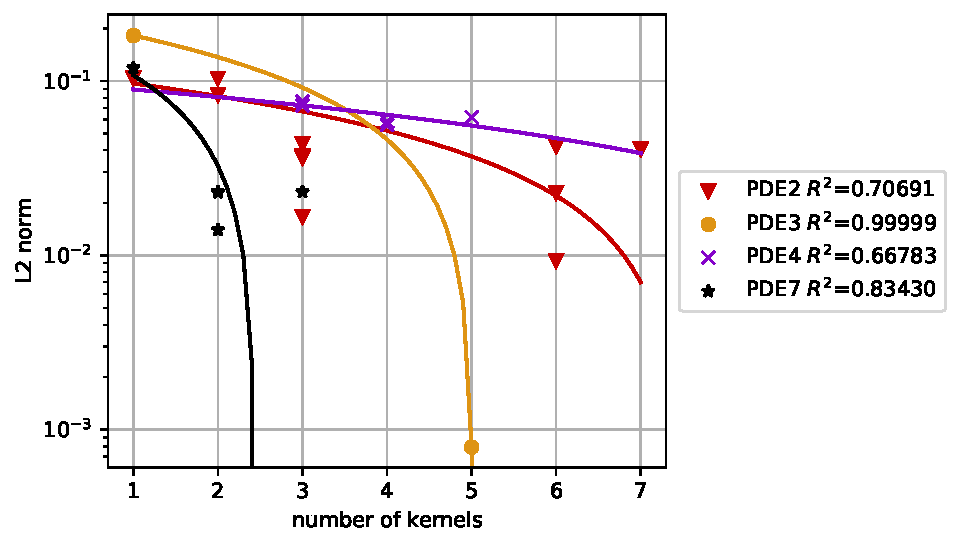
\includegraphics[width=\textwidth]{../../code/experiments/experiment_2/pde_2_3_4_7_kernels_vs_l2norm.pdf}
	}
	\unterschrift{Semi-logarithmic plot of the correlation between the L2 norm and the number of kernels. }{}{}
	\label{fig:pajade_pde2347_kernels_l2norm}
\end{figure}
It seems that JADE exploits some areas long enough so that it does not terminate due to convergence. Thus, the number of kernels is not increased, which leads to a poor approximation quality. A simple solution to mitigate this issue might be to adjust the parameters of the ``state-detector''. In this experiment, $minError = 0$ is used, however it might be beneficial to allow small changes in the function value and still terminate. \\
\textbf{\underline{Parameter Adaption: $minError$}} \\
In this ``sub-experiment'' the effect of increasing the $minError$ parameter is examined. Therefore, the same algorithm is rerun on the \gls{pde}s 2, 3, 4 and 7 at four different $minError$ levels. Again, 20 replications are done. It is expected that the average number of kernels is increased. Simultaneously, the approximation quality should become better. As expected, the average number of kernels in the solution gets increased. This is confirmed by the plot in figure \ref{fig:subexperiment_pde2347_minerror_kernelNR}. Figure \ref{fig:subexperiment_pde2347_minerror_l2norm} shows the connection between the median L2 norm and the $minError$. The distance to the analytical solution decreases on \gls{pde} 2 and 3. However, this does not improve the results of \gls{pde} 4 and 7, where the quality stays roughly on the same level. This is supported statistically by the Wilcoxon test in table \ref{tab:statistical_test_minError}.
\begin{figure}[h]
	\centering
	\begin{subfigure}[b]{0.5\linewidth}
		\centering
		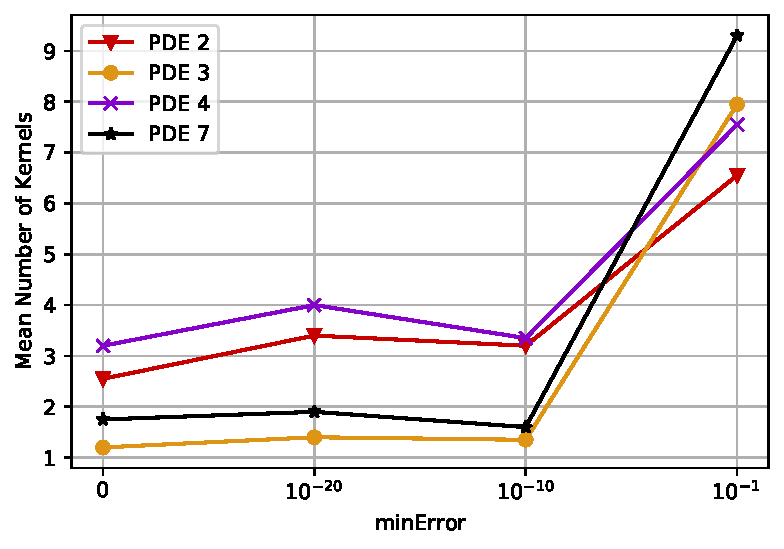
\includegraphics[width=1\textwidth]{../../code/experiments/misc/pde2347_minError_kernelNR.pdf}
		\caption{Plot of the mean number of kernels against the $minError$.}
		\label{fig:subexperiment_pde2347_minerror_kernelNR}
	\end{subfigure}% 
	%
	\begin{subfigure}[b]{0.52\linewidth}
		\centering
		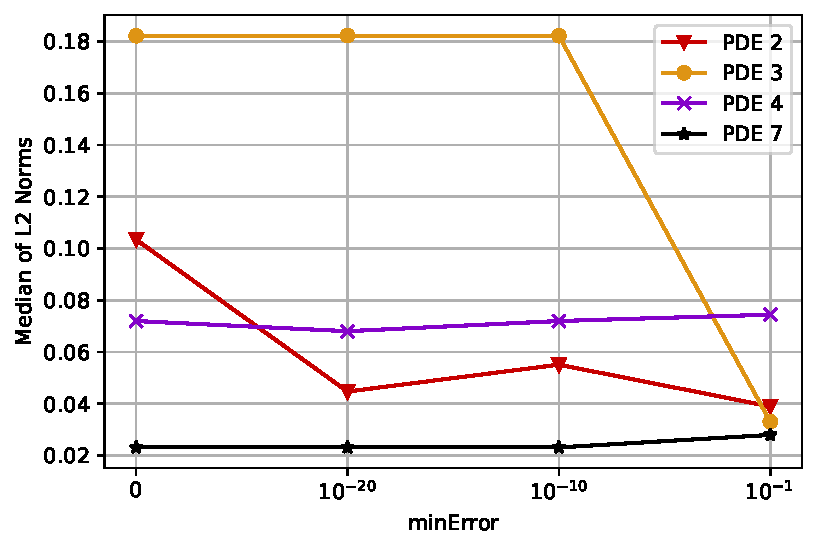
\includegraphics[width=1\textwidth]{../../code/experiments/misc/pde2347_minError_L2norm.pdf}
		\caption{Plot of the median L2 norm against the $minError$.}
		\label{fig:subexperiment_pde2347_minerror_l2norm}
	\end{subfigure}%
	\unterschrift{Comparison of $minError$ against the number of kernels and the achieved solution quality. }{}{}%
	\label{fig:subexperiment_pde2347_minerror}
\end{figure}
\begin{table}[h]
	\centering
	\noindent\adjustbox{max width=\linewidth}{
		\begin{tabular}{|c|c|c|c|c|l|}
			
			\hline
			\rowcolor[HTML]{\farbeTabA}
			
			Setup & \multicolumn{2}{|c|}{$minError = 0$; $10^6$ \gls{nfe}} & \multicolumn{2}{|c|}{$minError = 10^{-1}$; $10^6$ \gls{nfe}} & \\ \hline
			stat & mean & median & mean & median & Wilcoxon Test \\ \hline \hline
			\gls{pde} 2 & 0.0735 $\pm$ 0.0358 & 0.1034 & 0.0418 $\pm$ 0.0156 & 0.0389 & sig. better \\ \hline
			\gls{pde} 3 & 0.1731 $\pm$ 0.0395 & 0.1822 & 0.0455 $\pm$ 0.0406 & 0.0331 & sig. better \\ \hline
			\gls{pde} 4 & 0.0707 $\pm$ 0.0053 & 0.0720 & 0.0726 $\pm$ 0.0080 & 0.0744 & unsig. worse \\ \hline
			\gls{pde} 7 & 0.0513 $\pm$ 0.0442 & 0.0231 & 0.0287 $\pm$ 0.0045 & 0.0279 & unsig. undecided \\ \hline
			
		\end{tabular}
	}
	\unterschrift{Statistical comparison of the achieved L2 norm by paJADE with $minError = 0$ and $minError = 10^{-1}$ after $10^6$ \gls{nfe}.}{}{}
	\label{tab:statistical_test_minError}
\end{table}
Although the results on \gls{pde} 2 and 3 do get significantly better, the adaptive process with greater $minError$ introduces a larger spread of the results - both in the number of kernels and in the reached L2 norm. This can be seen in figure \ref{fig:subexperiment_pde2347_kernels_l2norm}. Compared to the same plot at $minError = 0$, the coefficient of determination $R^2$ is smaller, indicating a poor correlation and a greater spread. 
\begin{figure}[h]
	\centering
	\noindent\adjustbox{max width=0.8\linewidth}{
		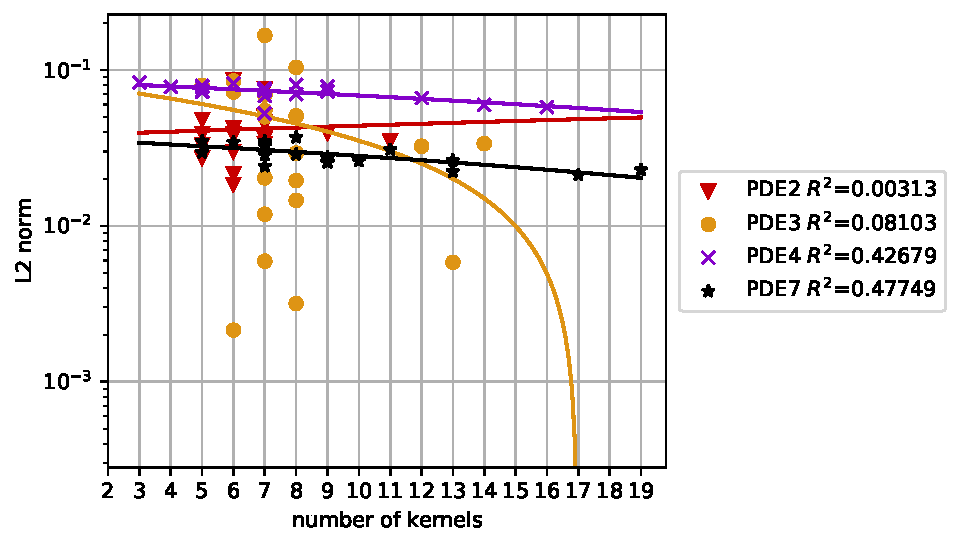
\includegraphics[width=\textwidth]{../../code/experiments/misc/pde2347_L2norm_kernelNR.pdf}
	}
	\unterschrift{Semi-logarithmic plot of the correlation between the L2 norm and the number of kernels. The results are produced with a $minError = 10^-1$ after $10^6$ \gls{nfe}.}{}{}
	\label{fig:subexperiment_pde2347_kernels_l2norm}
\end{figure}

\subsubsection{PDE 5}
The results presented in table \ref{tab:compare_mpj_mpja_10^6} show an interesting observation for the testbed problem 5. The mean L2 norm of the adaptive scheme is very large, but the median is slightly smaller than the median of the non-adaptive JADE. The Wilcoxon test reveals an insignificant difference, which hints that the adaptive scheme includes some very large outliers. This is demonstrated by comparing the box plots of both L2 norm distributions in figure \ref{fig:paJADE_pde5_l2norm_boxplot}. The same data is shown with and without the outlier. 
\begin{figure}[h]
	\centering
	\begin{subfigure}[b]{0.4\linewidth}
		\centering
		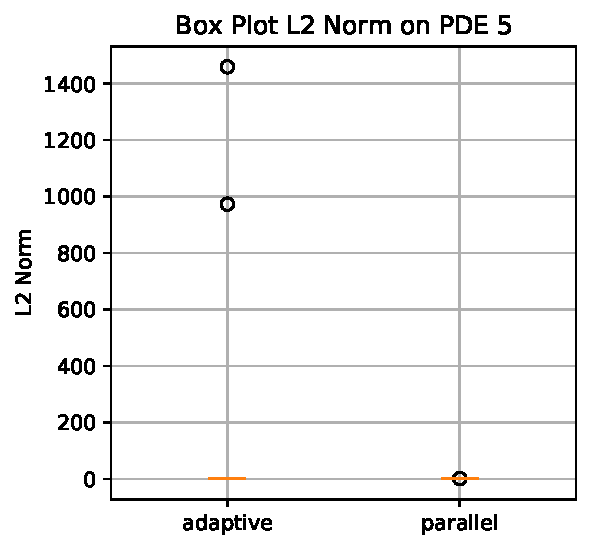
\includegraphics[width=1\textwidth]{../../code/experiments/experiment_2/pde5_L2_norm_boxplot.pdf}
		\caption{\gls{pde} 5 solution quality with outlier. }
		\label{fig:paJADE_pde5_l2norm_boxplot}
	\end{subfigure}% 
	%
	\begin{subfigure}[b]{0.39\linewidth}
		\centering
		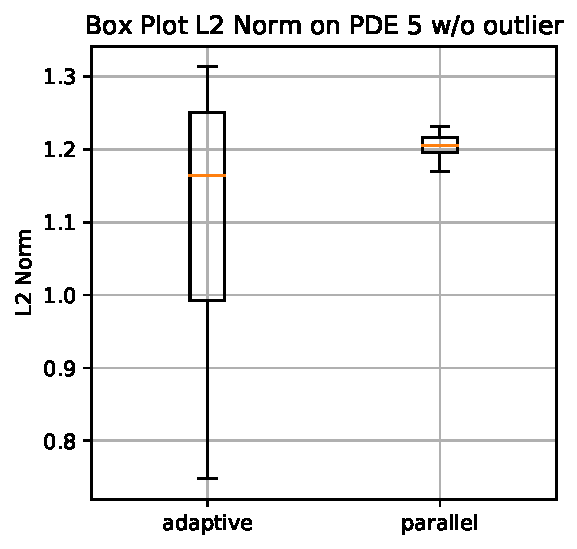
\includegraphics[width=1\textwidth]{../../code/experiments/experiment_2/pde5_L2_norm_boxplot_wo_outlier.pdf}
		\caption{\gls{pde} 5 solution quality without outlier. }
		\label{fig:paJADE_pde5_l2norm_boxplot_cleared}
	\end{subfigure}%
	%
	\unterschrift{Boxplot of solution quality on \gls{pde} 5 at $10^6$ \gls{nfe} with and without outliers. }{}{}%
	\label{fig:paJADE_pde5_l2norm_boxplot_comparison}
\end{figure}
In general, it can be said that the adaptive scheme exhibits a greater spread in the quality of the solution. 
\end{document}